%%%%%%%%%%%%%%%%%%%%%%%%%%%%%%%% Introducción:

\begin{frame}[fragile]{Agrupación Espacial:}{Propuestas I.}
  La agrupación espacial es un subconjunto espacial de agrupación. Este tipo
  de agrupamiento es relacionado, con frecuencia, a métodos gráficos.
  \begin{figure}
    \centering
    \begin{subfigure}[b]{0.3\textwidth}
      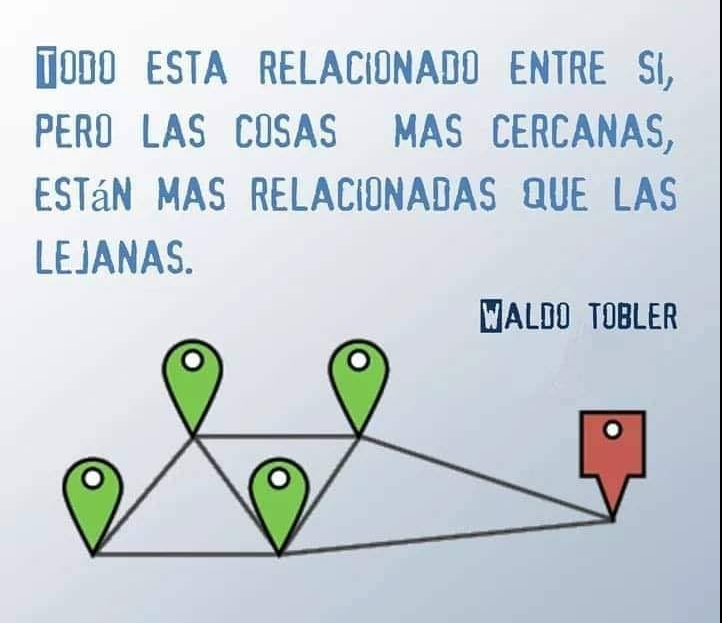
\includegraphics[width=\textwidth]{./Imagenes/LeyGeo.png}
      %\caption*{Redes Neuronales.}
    \end{subfigure}
    \begin{subfigure}[b]{0.2\textwidth}
      
\includegraphics[width=\textwidth]{./Imagenes/Waldo_Tobler_2007.jpg}
      %\caption*{K-means + Genéticos.}
    \end{subfigure}
    \caption*{1era ley de la geografía.}
  \end{figure}
  \textbf{Propuestas:}
  \begin{itemize}
  \item Zahn sugiere trabajar con un gráfico completo (con vértices cada elemento en el espacio),
    construir el árbol de expansión mínima y eliminar los ``bordes'' más largos comparando las
    longitudes de los arcos con la longitud promedio, eliminando aquellos con longitud mayor al
    doble de la longitud promedio.
  \end{itemize}
\end{frame}
